\chapter{Client}
\label{ch:client}
Hier beschreiben, was im folgenden Kapitel gemacht werden soll? Was ist das Ziel? Was muss vorbereitet werden?
Es soll der Client aufgebaut werden, welcher dann mit der REST-Schnittstelle kommuniziert.
\\ \\
Wir haben zwei Applikationen. Also muss man auch beide aufrufen können.
\\ \\
Ich habe eine Webseite auf Basis von Angular mit Angular-Material gebaut. - Mit der REST-Schnittstelle von API Connect
kommunizieren lassen (beide Endpunkte) - Zwei Smartphone-Apps aufgebaut,
welche die Webseite in einem WebViewer laden und anzeigen - Vorkehrungen getroffen, damit die Applikation in der Cloud
gebaut und gehostet werden kann (Toolchain, Git) - Bild mit schematischer Architektur (Markiert, was nun gemacht wird.
Rest ausgegraut)
\\ \\
1 - 2 Seiten

\colorbox{yellow}{Hier fehlt was}

\begin{figure}[h]
    \centering
    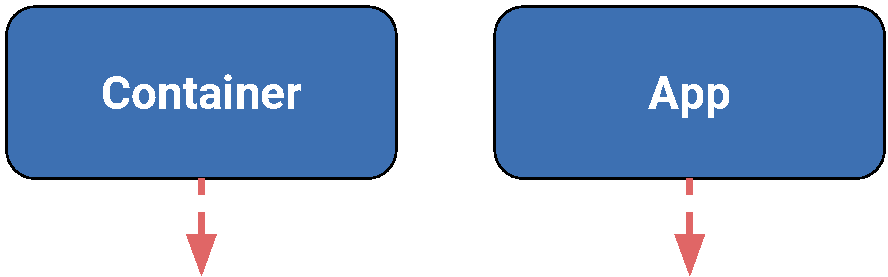
\includegraphics[scale=0.5]{images/kapitel_4/architektur_schematisch.pdf}
    \caption{Schematische Darstellung der Architektur}
    \label{fig:schematische_architektur_4}
\end{figure}